% IMPORTANT: PLEASE USE XeLaTeX FOR TYPESETTING
\documentclass[10pt]{beamer}

\usetheme{Darmstadt}%{default}
\usecolortheme{beaver}
\usepackage[T1]{fontenc} 
\usepackage[utf8]{inputenc}
\usepackage[french]{babel}
\usefonttheme{serif}
\usepackage{lmodern}
\usepackage{tcolorbox}
 % pour un pdf lisible à l'écran
 % il y a d'autres choix possibles 
\usepackage{pslatex}
% \usepackage{ctex, hyperref}
\usepackage{latexsym,amsmath,xcolor,multicol,booktabs,calligra}
\usepackage{graphicx,pstricks,listings,stackengine}
\usepackage{chemfig}

\usepackage{tabularx}
% meta-data

\author{Gabriel Le Doudic}
\institute{Préparation à l'agrégation de Rennes}
% \titlebackground{images/background}

\definecolor{aquamarine}{rgb}{0.5, 1.0, 0.83}
\definecolor{applegreen}{rgb}{0.55, 0.71, 0.0}	
\definecolor{cobalt}{rgb}{0.0, 0.28, 0.67}

\definecolor{definitionf}{RGB}{220,252,220}
\definecolor{definitionl}{RGB}{39,123,69}
\definecolor{definitiono}{RGB}{72,148,101}

\definecolor{propositionf}{RGB}{255,216,218}
\definecolor{propositionl}{RGB}{38,38,38}
\definecolor{propositiono}{RGB}{109,109,109}

\definecolor{theof}{RGB}{255,216,218}
\definecolor{theol}{RGB}{160,0,4}
\definecolor{theoo}{RGB}{221,65,100}

\definecolor{avertl}{RGB}{163,92,0}
\definecolor{averto}{RGB}{255,144,0}

\definecolor{histf}{RGB}{241,238,193}

\definecolor{metf}{RGB}{220,230,240}
\definecolor{metl}{RGB}{56,110,165}
\definecolor{meto}{RGB}{109,109,109}


\definecolor{remf}{RGB}{230,240,250}
\definecolor{remo}{RGB}{150,150,150}

\definecolor{exef}{RGB}{240,240,240}

\definecolor{protf}{RGB}{247,228,255}
\definecolor{protl}{RGB}{105,0,203}
\definecolor{proto}{RGB}{174,88,255}

\definecolor{grid}{RGB}{180,180,180}

\definecolor{titref}{RGB}{230,230,230}

\definecolor{vert}{RGB}{23,200,23}

\definecolor{violet}{RGB}{180,0,200}

\definecolor{copper}{RGB}{217, 144, 88}
%% CADRES

\newtcolorbox{defi}[1]{
	colback=applegreen!5!white,
  	colframe=applegreen!65!black,
	fonttitle=\bfseries,
  	title={#1}}
\newtcolorbox{Programme}[1]{
	colback=cobalt!5!white,
  	colframe=cobalt!65!black,
	fonttitle=\bfseries,
  	title={#1}}  
\newtcolorbox{Resultat}[1]{
	colback=theof,%!5!white,
	colframe=theoo!85!black,
  fonttitle=\bfseries,
	title={#1}} 
\usepackage{tikz}
\usepackage{array}
\usepackage[scientific-notation=true]{siunitx}
\usetikzlibrary{matrix}
\newcommand{\diff}{\mathrm{d}}

\title{Leçon : Conversion de Puissance Électromécanique}

% document body
\begin{document}
\begin{frame}{}
    \titlepage

    \begin{tabularx}{\textwidth}{l@{:\,\,}X}
        \textbf{Niveau} 	  & CPGE PSI\\
        \textbf{Prérequis} & Électromagnétisme \\
        & mécanique
    \end{tabularx}
\end{frame}

\begin{frame}
    \tableofcontents
\end{frame}

\section{Contacteur électromagnétique en translation}

\subsection{Principe de fonctionnement}

\begin{frame}{\insertsubsection}
    \begin{figure}
        \centering
        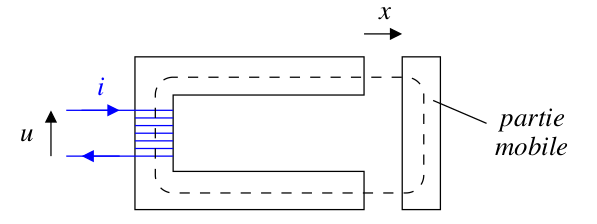
\includegraphics[width=1\textwidth]{ContacteurElectromagnetique.png}
        \caption{Contacteur électromagnétique}
    \end{figure}
\end{frame}

\subsection{Énergie magnétique emmagasinée}

\begin{frame}{\insertsubsection}
\textbf{Méthodologie}
\begin{enumerate}
    \item Théorême d'Ampère
    \item Conservation du flux du champ magnétique
    \item Expression du champ B  en fonction de l'ntensité
    \item Induction propre
    \item Énegie magnétique emmagasinée
\end{enumerate}
\end{frame}

\subsection{Force Électromagnétique}

\begin{frame}{\insertsubsection}
    \begin{figure}
        \centering
        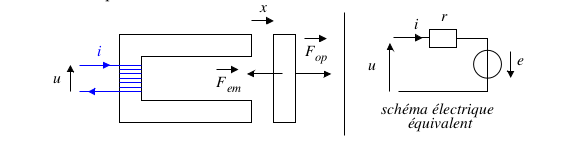
\includegraphics[width=1\textwidth]{ForceElectromagnetique.png}
    \end{figure}
    \pause
    Il faut noter que : 
    \begin{itemize}
        \item $F_M\propto i ^2$ c'est une force de rappel quelque soit le signe de $i$  et est nulle en moyenne dans le temps pour une excitation sinusoïdale
        \item Ce type de dispositif peut servir de contacteur électromagnétique permettant de commander la fermeture et l'ouverture d'un circuit électrique via le déplacement de la partie mobile, qui en l'absence de champ magnétique est ramenée à sa position initiale par l'intermédiaire d'un ressort.
    \end{itemize}
\end{frame}

\subsection{Généralisation}

\begin{frame}{\insertsubsection}
    On peut généraliser l'expression de la force : 

    \begin{equation}
        F = \left(\dfrac{\partial E}{\partial x}\right)_{\Phi}
    \end{equation}

    Pour un contacteur en rotation autour d'un axe fixe repéré par un angle $\theta$, on utilisera plutôt le moment des actions s'exerçant sur le contacteur : $\Gamma$
    \begin{equation}
        \Gamma = \left(\dfrac{\partial E}{\partial \theta}\right)_{\Phi}.
    \end{equation}
\end{frame}
\section{Machine à courant continu}
\subsection{Structure}
\begin{frame}{\insertsubsection}
    \begin{figure}
        \centering
        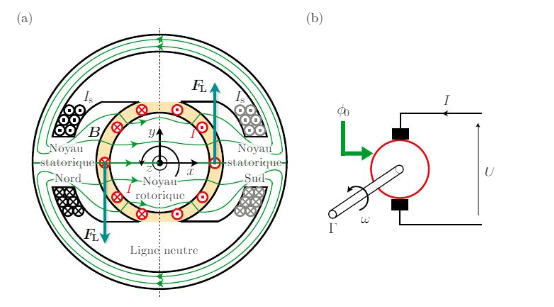
\includegraphics[width=1\textwidth]{StructureMCC.png}
        \caption{Physique expérimentale, Jolidon}
    \end{figure}
\end{frame}

\subsection{Rôle du collecteur}

\begin{frame}{\insertsubsection}
    \begin{figure}
        \centering
        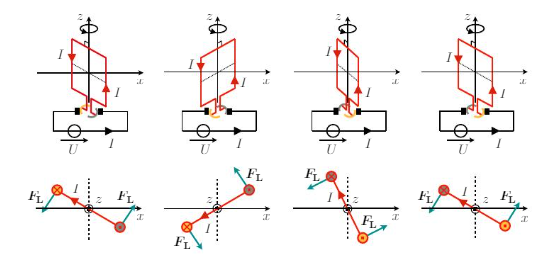
\includegraphics[width=1\textwidth]{RotorCollecteur.png}
        \caption{Physique expérimentale, Jolidon}
    \end{figure}
\end{frame}

\subsection{Constante électromécanique}
\begin{frame}{\insertsubsection}
    \begin{figure}
        \centering
        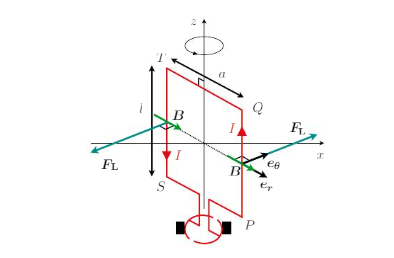
\includegraphics[width=1\textwidth]{SchemaPrincipe.png}
    \end{figure}
\end{frame}

\subsection{Point de fonctionnement}

\begin{frame}{\insertsubsection}
\begin{figure}[ht]
	\centering
	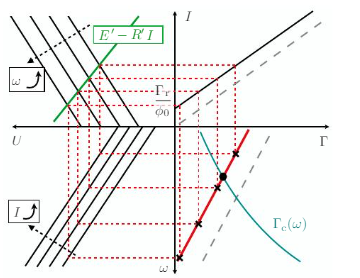
\includegraphics[width=.5\textwidth]{CaracteristiqueMCCPointDeFonctionnement.png}
	\caption{Caractéristique MCC, extrait du Jolidon}
\end{figure}
\end{frame}

\subsection{Bilan de puissance}
\begin{frame}{\insertsubsection}
\begin{figure}[ht]
	\centering
	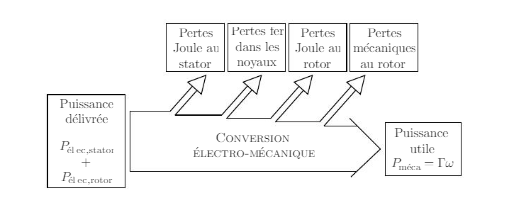
\includegraphics[width=1\textwidth]{BillanPuissance.png}
	\caption{Bilan de Puissance, extrait jolidon}
\end{figure}
\end{frame}
\section{Moteur synchrone}
\subsection{Structure}

\begin{frame}{\insertsubsection}
    \begin{figure}[ht]
	\centering
	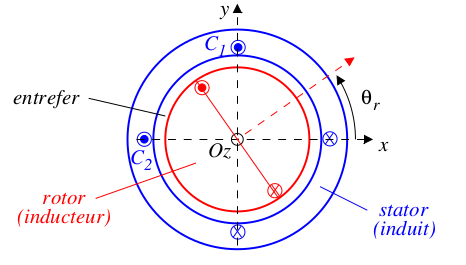
\includegraphics[width=.5\textwidth]{StructureMachinesynchrone.png}
	\caption{Schéma cours Naval}
\end{figure}
    \end{frame}

\subsection{Champ dans l'entrefer}

\end{document}